% ----------------------------------------------------------
% Introdução (exemplo de capítulo sem numeração, mas presente no Sumário)
% ----------------------------------------------------------
\chapter[Introduction]{Introduction}
%\addcontentsline{toc}{chapter}{Introduction}
% ----------------------------------------------------------

Attracting and retaining the interest of users are key factors for a software
system to achieve sustained
success~\cite{subramaniam2009determinants,delone2003delone}. In this context,
software development teams that do not address issues that are reported by
users, lead their software system to remain stagnant and lose credibility. We
broadly use the term issue to either describe a \textit{new feature}, a
\textit{bug}, or an \textit{enhancement} that should be addressed in a software
system~\cite{giuliano2008}.

Within a globalized world, in which technology has fostered geographically
distributed software development~\cite{herbsleb2003empirical}, software
development teams use \textit{Issue Tracking Systems} (ITS, e.g., Bugzilla) to
coordinate their tasks.\smartfoot{\url{https://www.bugzilla.org/}} Users can use
ITSs to report issues within software systems. To do so, these users must fill
in a report that contain information about the issue (\eg the description and
severity of the issue). 

The basic lifecycle of an issue is comprised of four steps. First, an issue is
{\em reported} to the software project's team. Once reported, an issue has to be
\textit{triaged}, \ie the team members must decide whether an issue should be
addressed or not. In case that an issue is deemed to be worth addressing, a team
member with the right expertise is assigned to the issue~\cite{Anvik2006}. After
being triaged, an issue is \textit{addressed} by its assignee, \ie a solution is
provided and tested for that issue. Finally, the addressed issue is integrated
and delivered to the end user through an official release of the software
system.  Issues may also be \textit{reopened} if the solution that was provided
to the issue is found to be incorrect. In this case, a new solution has to be
provided, tested, and integrated.

\section{Problem Statement} \label{sec:problem}

Once an issue is \textit{addressed}, (\ie a solution for that issue is provided
and tested), such an addressed issue may still have a delay before reaching users.
For instance, Jiang~\etal~\cite{Jiang2013} find that a reviewed code change
might take an additional 1-3 months to be integrated into the Linux kernel.
Users care most about when addressed issues will be available in the software
system (so they can benefit from those addressed issues). We use the term
\textit{delivery delay} to refer to the delay that addressed issues suffer prior
to their delivery to end users. 

Delivery delay can be frustrating to users. For example, in a recent issue
report of the Firefox system, a user asks: \textit{``So when does this stuff get
added? Will it be applied to the next FF23 beta? A 22.01 release?
Otherwise?''}.\smartfoot{\url{https://bugzilla.mozilla.org/show_bug.cgi?id=883554}}
Moreover, in the open source software community, developers may also be
motivated to contribute because they want to see a particular feature available
in the software system in a timely manner~\cite{Jiang2013}. In such a case,
delivery delays frustrate these contributors. 

The present thesis is an effort to reduce the lack of empirical understanding as
to why addressed issues suffer delivery delay before being available to users. A
good understanding of such delays will help software projects reduce such
undesirable delays.

\section{Current Research Limitations}

Prior research has investigated the time that is needed to triage and address
issues~\cite{Anvik2005, Anbalagan2009, Giger2010, Kim2006, Marks2011, Weib2007,
Zhang2013}. Such research provides valuable insight on which issues should be
prioritized. For example, issues might be addressed earlier given the estimated
time that they are likely to take to be addressed. Nevertheless, after an issue
is addressed, such an addressed issue may still require considerable time to be
delivered to users.

Another line of prior work has investigated the integration stage of software
development. Jiang~\etal~\cite{Jiang2013} studied the likelihood of patches that
were submitted to the Linux Kernel project of being integrated in the main code
base. On the other hand,
Choetkiertikul~\etal~\cite{riskyissues2015a,riskyissues2015b} studied the risk
of issues of postponing the shipment of new releases. However, the investigation
of: {\em (i)} what leads addressed issues to suffer delivery delay even when
releases are shipped and {\em (ii)} the impact of release development strategies
on such delays remain as open challenges.

\section{Thesis Proposal} \label{sec:thesis_overview}

\begin{sloppypar}
The general research question that is investigated in this thesis is {\em
\underline{what leads addressed issues to suffer delivery delay?}}
\end{sloppypar}

\begin{figure}[t]
	\centering
	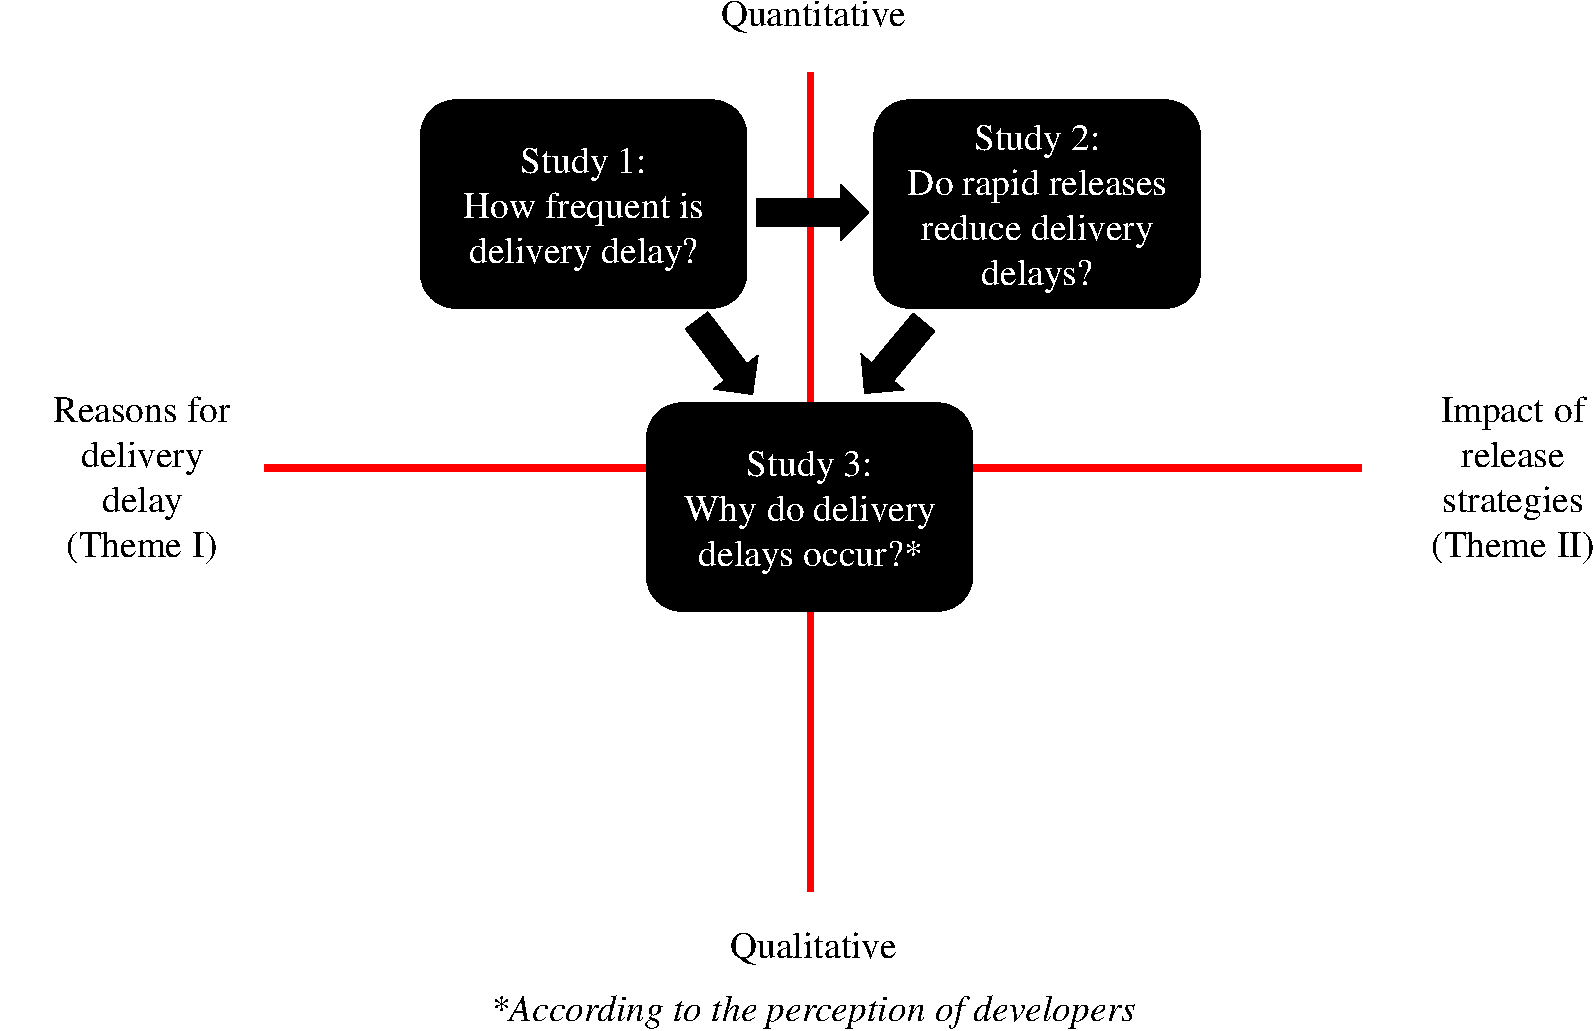
\includegraphics[width=0.90\textwidth,keepaspectratio]
	{chapters/chapter1/figures/thesis_overview.pdf}
	\caption{An overview of the scope of the thesis.}
	\label{fig:thesis_overview}
\end{figure}

\hyperref[fig:thesis_overview]{Figure}~\ref{fig:thesis_overview} provides an
overview of the scope of this thesis. The scope shows the studies that we
perform towards our general research question. The studies that are performed in
this thesis are grouped into two {\em themes}. {\em
Theme~I}\parts{pt:deliverydelay} is regarding {\em reasons for delivery delay},
which encompasses \hyperref[st:study1]{Studies}~\ref{st:study1} and part of
\hyperref[st:study4]{Study}~\ref{st:study4}. In {\em
Theme~II}\parts{pt:rapidreleases}, we investigate the {\em impact of release
development strategies} on the delivery delay of addressed issues
(\hyperref[st:study3]{Study}~\ref{st:study3} and part of
\hyperref[st:study4]{Study}~\ref{st:study4}). We present the motivation of
performing each study of this thesis in the subsections below.

\subsection{Study~1---How frequent is delivery delay?}

\study{st:study1} 33\% of the code patches that are submitted to resolve issues
of the Linux kernel take 3 to 6 months to be accepted into an official
release~\cite{Jiang2013}. Such observation hints that the integration stage may
introduce non-trivial delays before delivering addressed issues. Since there is
a lack of empirical studies that investigate the frequency of delivery delays of
addressed issues, we perform a study using 20,995 addressed issues of the
ArgoUML, Eclipse, and Firefox projects in
\hyperref[st:study1]{Study}~\ref{st:study1}. Our main goal is to analyze {\em
(i)} how frequent delivery delays occur and {\em (ii)} which factors may impact
delivery delay according to our studied data.
%\subsection{Study~2---What leads to prolonged delivery delays?}
%\study{st:study2} 

Also in this study, we investigate delivery delays that are considered to be
{\em prolonged} in a particular project. For example, supposing that addressed
issues are usually delivered within 60 days on a particular project, a delivery
delay of 120 days would be abnormal for that project. This investigation is
important because prolonged delays can be more frustrating to users, since they
are not used to such delays.

\subsection{Study~2---Do rapid releases reduce delivery delays?}

\study{st:study3} After an issue is addressed, a release must be shipped in
order to end users experience the addressed issue. The process of shipping
releases varies according to the release cycles that are adopted by the project
team.  Recently, many organizations have shifted to shorter release cycles (\eg
6 weeks rather than 12 months) with the allure of delivering software issues
more quickly to end users. For instance, Firefox, Chrome, and Facebook have
adopted shorter release cycles to ship major releases. In
\hyperref[st:study3]{Study}~\ref{st:study3}, we empirically study whether
shorter release cycles quicken the delivery of addressed issues to end users. We
set out to empirically compare the traditional and rapid releases of the Firefox
project regarding the delivery delay of addressed issues. In total, we study 71,114
issue reports.

\subsection{Study~3---Why do delivery delays occur?}

\study{st:study4} In our other studies
(\hyperref[st:study1]{Studies}~\ref{st:study1} and \ref{st:study3}), we
quantitatively investigate the delivery delay of addressed issues. We perform
several statistical analyses based on the data that is publicly available on the
ITSs and {\em Version Control Systems} (VCSs) of our subject projects. Nevertheless, to better understand the
reasons as to why delivery delays occur, we survey 37 participants from the
ArgoUML, Firefox, and Eclipse projects about the delivery delay of addressed
issues. We also perform follow up interviews with four participants to get
deeper insights about the responses that we receive.
\hyperref[st:study4]{Study}~\ref{st:study4} help us to {\em (i)} reach
additional insights that could not be possible by only performing quantitative
analysis and {\em (ii)} verify to which extent our participants agree with our
findings from the quantitative studies. 

\section{Thesis Contributions}

We outline the contributions of this thesis below. The contributions are grouped
by their respective study.

\subsubsection*{Study~1---How frequent is delivery delay?}

\begin{itemize}

	\item Despite being addressed well before an upcoming release, 34\% to
		60\% of the addressed issues are not integrated in more than one
		release in the ArgoUML and Eclipse projects. Furthermore, 98\%
		of the Firefox project issues had their integration delayed by
		at least one release
		(\hyperref[ch:study12]{Chapter}~\ref{ch:study12}).

	\item Heuristics that estimate the effort that teams invest in
		fixing issues are the most influential factors to
		estimate delivery delay in terms of number of releases
		(\hyperref[ch:study12]{Chapter}~\ref{ch:study12}).

	\item Surprisingly, \textit{priority} and \textit{severity} have little
		impact on delivery delay. Indeed, 36\% to 97\% of priority P1
		addressed issues were delayed by at least one release
		(\hyperref[ch:study12]{Chapter}~\ref{ch:study12}).

	\item Shorter delivery delays are associated with issues that are
		addressed during more controlled stages (\eg a code freeze
		stage) of a given release cycle
		(\hyperref[ch:study12]{Chapter}~\ref{ch:study12}).

	\item The time at which issues are addressed and the resolvers
		of the issues have great impact on estimating the
		delivery delay (in terms of days) of an issue
		(\hyperref[ch:study12]{Chapter}~\ref{ch:study12}).

	\item The time at which an issue is addressed (queue position), the
		integration workload (in terms of the backlog of addressed
		issues), and the heuristics that estimate the effort that teams
		invest in fixing issues (fixing time per resolver), are the most
		influential attributes for issues that have a prolonged delivery
		delay (\hyperref[ch:study12]{Chapter}~\ref{ch:study12}). 

	\item Our models that identify addressed issues that have a prolonged
		delivery delay outperform random guessing and Zero-R models,
		obtaining AUC values of 0.82~to~0.96
		(\hyperref[ch:study12]{Chapter}~\ref{ch:study12}).

\end{itemize}

\subsubsection*{Study~2---Do rapid releases reduce delivery delays?}

\begin{itemize}

	\item Although issues tend to be addressed more quickly in rapid
		release cycles, addressed issues tend to be integrated into
		consumer-visible releases more quickly in traditional
		release cycles. However, a rapid release cycle may improve the
		consistency of the delivery rate of addressed issues
		(\hyperref[ch:study34]{Chapter}~\ref{ch:study34}).

	\item The total time that is spent from the issue report date to its
		integration into a release is not significantly different
		between traditional and rapid releases
		(\hyperref[ch:study34]{Chapter}~\ref{ch:study34}).

	\item In traditional releases, addressed issues are less likely to be
		delayed if they are addressed recently in the backlog. On the
		other hand, in rapid releases, addressed issues are less likely
		to be delayed if they are addressed recently in the current
		release cycle (\hyperref[ch:study34]{Chapter}~\ref{ch:study34}). 
\end{itemize}

\subsubsection*{Study~3---Why do delivery delays occur?}

\begin{itemize}

	\item The perceived reasons for delivery delay of addressed issues are
		primarily related to activities such as development, decision
		making, team collaboration, and risk management
		(\hyperref[ch:study34]{Chapter}~\ref{ch:study34}). 

	\item  The dependency of issues on other projects and team workload are the main
		perceived reasons to explain our data about delivery delay in
		general (\hyperref[ch:study34]{Chapter}~\ref{ch:study34}).  

	\item The allure of delivering addressed issues more quickly to users is
		the most recurrent motivator for switching to a rapid release
		cycle. In addition, the allure of improving management
		flexibility and quality of addressed issues are other advantages
		of rapid releases that are perceived by our participants
		(\hyperref[ch:study34]{Chapter}~\ref{ch:study34}).

	\item Integration rush and the increased time that is spent on polishing
		addressed issues (during rapid releases) emerge as one of the
		main explanations as to why traditional releases may have
		shorter delivery delays.
		(\hyperref[ch:study34]{Chapter}~\ref{ch:study34}).

\end{itemize}

\section{Thesis Organization}

The remainder of this thesis is organized as follows. In
\hyperref[ch:background]{Chapter}~\ref{ch:background}, we provide the background
material to the reader. In \hyperref[ch:study12]{Chapter}~\ref{ch:study12},
\hyperref[ch:study34]{Chapter}~\ref{ch:study34}, and
\hyperref[chapter6]{Chapter}~\ref{chapter6}, we present
\hyperref[st:study1]{Studies}~\ref{st:study1},~\ref{st:study3},
and~\ref{st:study4}, respectively. In
\hyperref[chapter7]{Chapter}~\ref{chapter7}, we present related research with
respect to this thesis. Finally, in
\hyperref[ch:conclusions]{Chapter}~\ref{ch:conclusions}, we draw our
conclusions.

